\documentclass[../main.tex]{subfiles}

\begin{document}

\chapter{Trends and variability in Antarctic Ice}
\label{chap:ice_behaviour}
Before we get into any complicated analysis we will start with the simplest thing we can. Describing and understanding the trends in Antarctic Ice in our datasets. We will start this by looking at Antarctic sea-ice, first looking at concentrations and extents before briefly discussing the thickness and volume of the ice. Then we will discuss in some detail, our understanding of land ice in Antarctica. And finally we will compare the two datasets and look at the trends and variability's of the two datasets combined.

For each dataset we look at we want to look at the following things. How the total ice has changed over time. How this changes with different temporal frequencies. How this also changes if we remove seasonal patterns or trends. What the seasonal patterns and trends we see in Antarctic Ice are. How significant these behaviours are. And how this all might impact the way we carry out further research. Finally we will want to acknowledge any shortcomings in our understanding of Antarctic ice and what the associated ramifications might be.



\section{Sea ice}
\subsection{Sea ice concentration}
\begin{figure}[H]
    \centering
    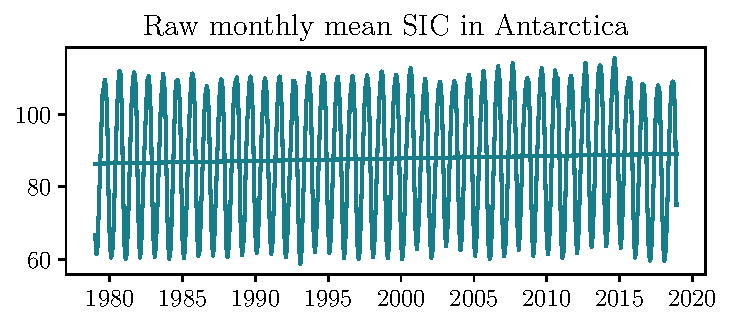
\includegraphics{images/timeseries/SIC/raw_monthly_1_raw.pdf}
    \caption{Raw mean Antarctic Sea Ice concentration from 1979 to 2019.\textcolor{red}{[WIP update with new plot}}
    \label{fig:sic_timeseries}
\end{figure}

\subsection{Sea ice thickness}
\subsection{Sea ice volume}


\section{Land Ice}
\subsection{Land Ice thickness}
\subsection{Land Ice volume}

\section{Combined Ice dataset}


\section{Implications for further research}

\section{Limitations}

\end{document}